% setup the document and include packages
\documentclass{article}[12pt]
\usepackage{graphicx}
\usepackage{amsmath}
\usepackage{amssymb}
\usepackage{cancel}
\usepackage{ntheorem}
\usepackage{algorithm2e}
\usepackage{float}
\usepackage{caption}
\usepackage{fancyvrb}
\usepackage[dvipsnames]{xcolor}
\usepackage[section]{placeins}
\usepackage[toc,page]{appendix}
\usepackage{hyperref}
\usepackage{subfig}
\usepackage{hyperref}
\hypersetup{
    colorlinks=true,
    linkcolor=blue,
    filecolor=magenta,      
    urlcolor=cyan,
}
\urlstyle{same}

\makeatletter
\def\BState{\State\hskip-\ALG@thistlm}
\makeatother

% define Continue for algorithms
\SetKw{Continue}{continue}

% redefine QED symbol
\renewcommand{\qedsymbol}{\rule{0.7em}{0.7em}}

\usepackage{mathtools}
\DeclarePairedDelimiter\ceil{\left\lceil}{\right\rceil}
\DeclarePairedDelimiter\floor{\left\lfloor}{\right\rfloor}

% define lemma and result theorem-styled sections
\newtheorem{lemma}{Lemma}[section]
\newtheorem{result}{Result}[section]

% setup paths for images
\graphicspath{ {plots/} }

% Don't print the semicolon in algorithms
\DontPrintSemicolon

% define the title that will be used in the report
\title{Project Title \\ CS 598 PS - ML in Signal Processing}
\author{
Ryley Higa \\ higa2@illinois.edu
\and 
Christian Howard \\ howard28@illinois.edu
\and
Sameer Manchanda \\ manchan2@illinois.edu
}
\date{} % don't set a date because we don't need this shit


% start the document
\begin{document}
   
   % create the title page 
   \maketitle
   \begin{abstract}
   A set of classifiers were built that could be used to predict if an individual has Major Depression given fMRI data about them performing a set of tasks. To accomplish this task, a dense fMRI dataset was coarsened via a local voxel averaging scheme and then features were discovered using Principal Component Analysis (PCA) and Non-negative Matrix Factorization (NMF). Using the new feature representations, classifiers were constructed using the following approaches: Random Forests, Gaussian Discriminant Analysis (GDA), and a Deep Neural Network (DNN). All of the above classification methods had high testing accuracy. This high accuracy was interesting and appears to stem from the feature representation causing the reduced data to be very separable with respect to their classes.
   \end{abstract}
   \newpage
   
   % create table of contents on separate page
   \tableofcontents
   \newpage
   
   % describe the background of the project
   \section{Project Background}
   \subsection{Dataset Description}
   The dataset used within this analysis was obtained from OpenfMRI. It contains data from 19 individuals with Major Depressive Disorder and 20 individuals with no mental illness. fMRI data was then collected for all these individuals while they did a set of tasks related to listening to different clips of audio. The resulting dataset is a time series information of Blood Oxygenation at a dense point cloud of locations within the patients’ brains.
   
   \subsection{What is fMRI Data?}
   fMRI stands for Functional Magnetic Resonance Imaging. The idea of how this works is that tissue is placed within a strong magnetic field. To help capture a picture of the tissue, radio waves are sent into the tissue. Blood that is deoxygenated will then reflect the waves in a manner that can be processed by sensors and algorithms to generate a fMRI dataset. Figure \ref{fig:brainSlice} shows example visualizations of some subset of the fMRI data used within this problem.
   
   \begin{figure}[!htb]
   	\centering
   	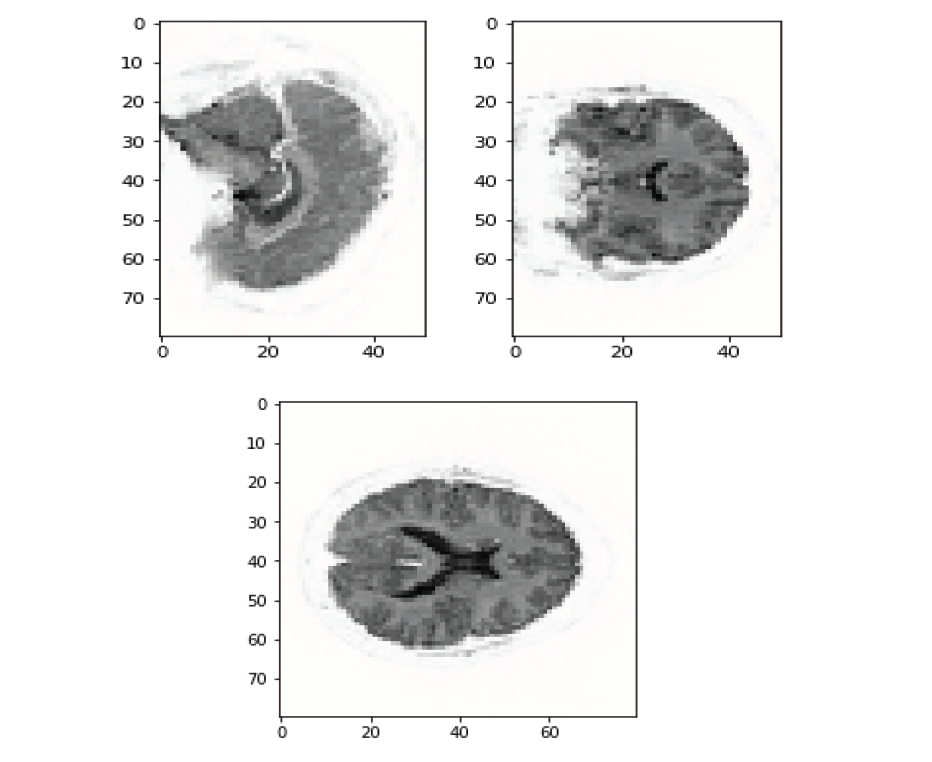
\includegraphics[scale=0.7]{brain_slices}
   	\caption{Image slices of the Intensities of Blood Oxygenation levels of some brain at the initial time}
   	\label{fig:brainSlice}
   \end{figure}
   
   \subsection{Problem Being Investigated}
   
   
   \section{Problem Solution}
   \subsection{Unsupervised Learning}
   The objective of our unsupervised learning tasks was to spatially reduce the dimensions of the fMRI dataset. The coarsened fMRI dataset consists of $180$ measurement sessions each session containing a time series of $3$-dimensional points clouds where each point cloud consists of $16$ by $16$ by $10$ spatial dimensions corresponding to the blood oxygen activation at the measured coordinate in the brain.  For every measurement session, we had $435200$ measured samples in total which we wanted to reduce so that the sessions can be easily classified as belonging to patients in the control group or to patients in the major depressive disorder group. We decided that only reducing the dataset in the spatial dimensions was the best method to reduce the overall dimensions of our dataset because we observed that sequential variance was more important than spatial variance for fMRI classification. 
   The two methods we used to reduce the dimensions were PCA and NMF. NMF was a natural choice for dimensionality reduction since the blood oxygen levels were all non-negative values. 
   \subsection{Supervised Learning}
   \subsubsection{Gaussian Discriminant Analysis}
   As a fairly straight forward model for classification, Gaussian discriminant functions with full covariance estimates were used. The idea is to perform a Maximum a Posteriori (MAP) estimate of which class $\omega^*$, out of a set of classes $\lbrace \omega_k \rbrace$, is best representative given some input $x$. This can be expressed as:
   
   \begin{align*}
   \omega^* &= \arg \max_{\omega_k} g_k(x)
   \end{align*}
   
   where $g_k(\cdot)$ is the discriminant function for class $\omega_k$. For a full Gaussian estimate, $g_k(\cdot)$ can be readily written as:
   
   \begin{align*}
   g_k(x) &= a_k + b_k^T x + x^T C_k x \\
   a_k &= \log P(\omega_k) - \frac{1}{2} \log \left| \Sigma_k \right| - \frac{1}{2} \mu_k^T \Sigma_k^{-1} \mu_k \\
   b_k &= \Sigma_k^{-1} \mu_k \\
   C_k &= -\frac{1}{2} \Sigma_k^{-1}
   \end{align*}
   
   where $\mu_k$ and $\Sigma_k$ are the expected value and covariance for $x$ given we are in class $\omega_k$. Using this representation, a classifier can be efficiently learned and used to obtain quadratic decision boundaries.
   
   
   \subsubsection{Random Forests}
   \subsubsection{Deep Neural Networks}
   Since deep convolutional neural networks have recently achieved state-of-the-art performance on various pattern recognition and classification tasks, we wanted to compare the performance of CNNs versus random forest classifiers and Gaussian discriminate analysis. The architecture of the CNN is shown in \textbf{figure 2}.  It was suggested by Sarraf and Tofighi \textbf{CITE!!!!!} that LeNet-5, a network first designed by LeCunn et Al. \textbf{CITE!!!!!} for handwritten digit classification, could be trained with minimal to no changes on fMRI data and still produce 96.86% accuracy on tasks such as Alzheimer classifcation. In practice, we did make changes to LeNet-5 including the inclusion of batch normalization layers to help the network converge faster, and combining the two 2x2 subsamplng layers into one 4x4 max pooling layer because it gave the network better accuracy on the validation data for our depression classification task. Overall, our network is fairly similiar to LeNet-5 with the inclusion of two convolutional layers, for instances of ReLU hiddden activation functions, and lastly two fully-connected layers. The loss function that was chosen was the sigmoid loss, which is fairly standard for binary classification tasks.  
   \begin{figure}[!htb]
   	\centering
   	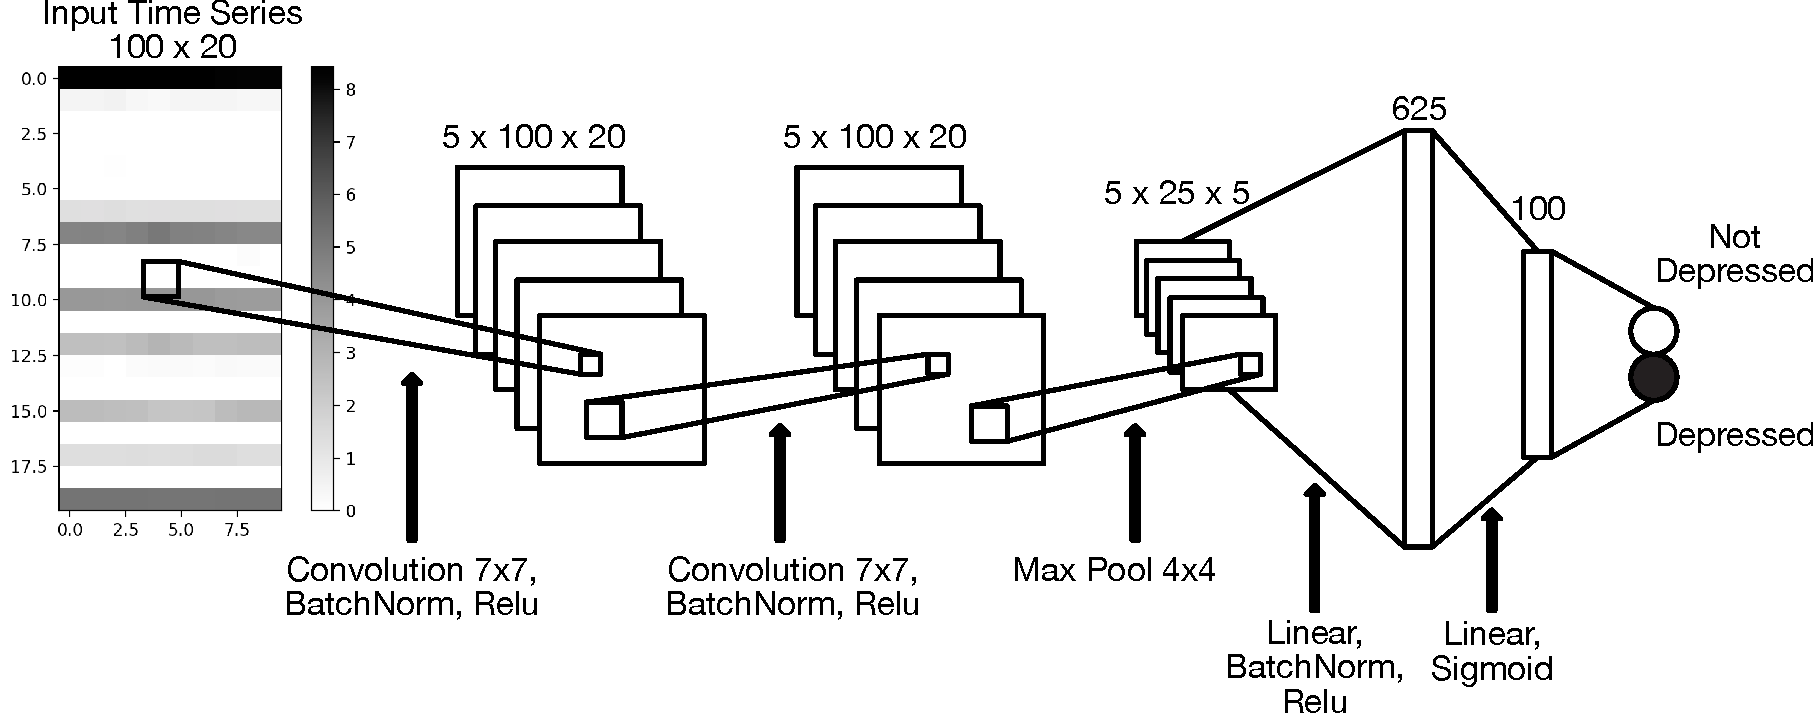
\includegraphics[width=4in]{DNN_diagram_annotated.pdf}
   	\caption{Deep Neural Network Configuration}
   	\label{fig:dnnConfig}
   \end{figure}
   
   
   \subsection{Numerical Results}
   After performing the necessary coarsening and dimensionality reduction, a set of models were built for predicting if someone has Major Depressive Disorder based on their fMRI data.  All models performed well but, as \textbf{Figure 4} shows, their success for a given number of features was dependent on the modeling approach. 
   
   Random Forests proved to not only perform well for the provided NMF features, but was very fast to compute. GDA performed well using PCA feature as the number of PCA features increased and was also very efficient to compute. Now while the Deep Neural Network required more computational complexity to train, it showed great performance as well. As can be seen in Figure 4, GDA required the most number of features to achieve greater than 90\% classification performance while the Random Forests and Deep Neural Network needed only 5 or more features to achieve high accuracy.
   
   \newpage
   \begin{thebibliography}{9}
   	\bibitem{labook} 
   	Gene H. Golub, Charles F. Van Loan. 
   	\textit{Matrix Computations 4\textsuperscript{th} Edition}. 
   	The John Hopkins University Press, Baltimore, Maryland, 2013.
   	
   	\bibitem{fdft} 
   	Henrik V. Sorensen, C. Sidney Burrus.
   	\textit{Efficient Computation of the DFT with Only a Subset of Input or Output Points}.
   	IEEE Transactions on Signal Processing, Volume: 41, Issue: 3, pgs. 1184 - 1200, Mar 1993.
   \end{thebibliography}
   
   
   \newpage
\begin{appendices}

\end{appendices}   
   
   
   
\end{document}